
\chapter{Зубчатые элементарные передачи}
\label{ch:gears}

\newthought{Механическая система ОЭП} выполняет функцию позиционирования различных элементов оптической системы в пространстве с заданной точностью.
Вид движения оптических элементов зависит от их назначения, но в большинстве случаев можно выделить вращательное и поступательное движения.
Передача энергии в механической системе ОЭП осуществляется различными механизмами.

\noindent
\textsc{Механизм}\marginnote{\allcaps{МЕХАНИЗМ}} --- система тел, предназначенная для преобразования движения одного или нескольких твердых тел в требуемое движение других твердых тел.

\noindent
\textsc{Кинематическая пара}\marginnote{\allcaps{КИНЕМАТИЧЕСКАЯ ПАРА}} --- соединение двух соприкасающихся звеньев, допускающих их относительное движение.

\noindent
\textsc{Кинематическая цепь}\marginnote{\allcaps{КИНЕМАТИЧЕСКАЯ ЦЕПЬ}} --- система звеньев, связанных между собой кинематическими парами.

\noindent
\textsc{Зубчатая элементарная передача}\marginnote{\allcaps{ЗУБЧАТАЯ\break ЭЛЕМЕНТАРНАЯ\break ПЕРЕДАЧА}} --- механизм, состоящий из зубчатых колёс, назначение которого --- передача вращательного движения между валами, обычно с изменением скоростей вращения или направления и характера движения.

\noindent
ГОСТ 16530-83: \textsc{зубчатое колесо}\marginnote{\allcaps{ЗУБЧАТОЕ КОЛЕСО}}~--- зубчатое звено с замкнутой системой зубьев, обеспечивающее непрерывное движение другого зубчатого звена.

\begin{marginfigure}
	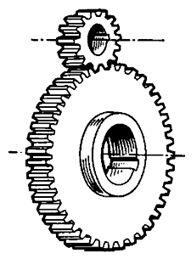
\includegraphics[width=0.6\linewidth]{osi1.png}
\end{marginfigure}

Классификация передач осуществляется по различным признакам, основные из которых:
\begin{itemize}
	\item передаточное отношение: постоянное или переменное;
	\item характер движения: меняет или не меняет направление;
	\item взаимное расположение осей валов: параллельное, пересекающиеся и скрещивающиеся;
	\item характер изменения скорости (замедление или ускорение);
	\item вид зубьев колес: прямозубые, косозубые, с внешним или внутренним зацеплением.
\end{itemize}

\begin{marginfigure}
	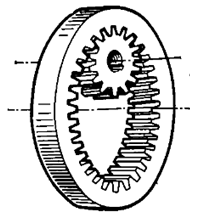
\includegraphics[width=0.6\linewidth]{osi2.png}
\end{marginfigure}

За начальную, предшествующую зубчатой, можно принять передачу посредством двух соприкасающихся, вращающихся без проскальзывания окружностей диаметра $ d_1 $ и $ d_2 $.
В этом случае обеспечивается постоянное передаточное отношение $ i_{12}=\omega_1 / \omega_2 = d_1 / d_2 $. 
В подобных реальных фрикционных передачах требуется большая сила прижатия цилиндров.

\begin{figure*}[h!]
	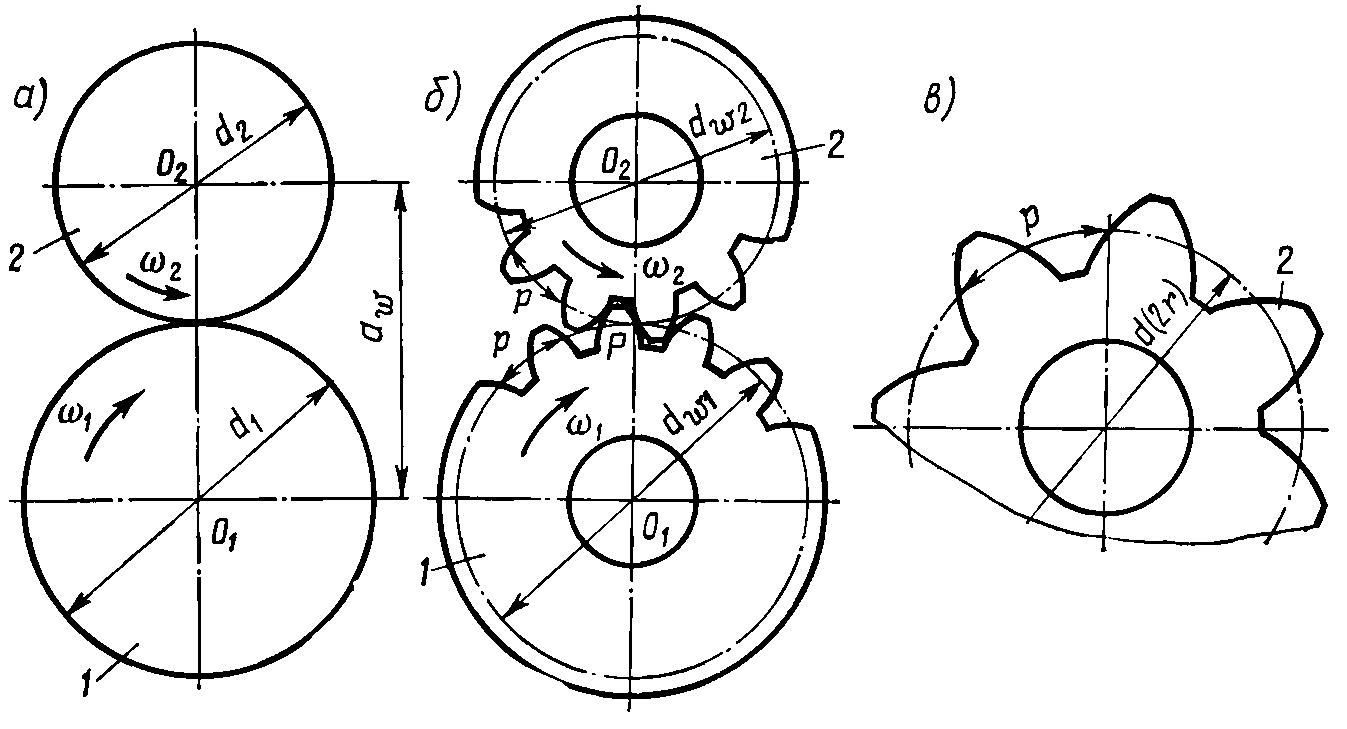
\includegraphics[width=\textwidth]{ZK_nachalo.png}
	\caption{Начальные окружности}
	\label{pic:ZK_nachalo}
\end{figure*}

\begin{marginfigure}
	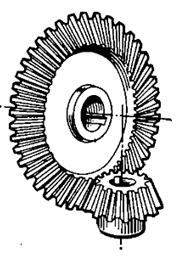
\includegraphics[width=0.7\linewidth]{osi3.png}
\end{marginfigure}

\begin{marginfigure}
	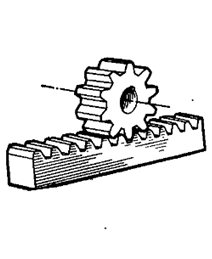
\includegraphics[width=0.8\linewidth]{osi4.png}
\end{marginfigure}

\begin{marginfigure}
	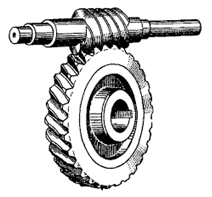
\includegraphics[width=0.8\linewidth]{osi6.png}
\end{marginfigure}

Проскальзывание можно полностью устранить, если на ободах цилиндров нарезать зубья.
В процессе работы зубья ведущего колеса \textsc{1} входят во впадины, давят на зубья колеса 2 и поворачивают его, преодолевая полезный момент сопротивления и силы трения в опорах и между зубьями.
При наличии зубьев сила прижатия колёс, как у фрикционных передач, не нужна, поэтому значительно сокращается давление на опоры.
При идеально точном изготовлении зубчатая передача должна воспроизводить такую же передачу вращения, как и посредством соприкасающихся окружностей.

Такие соприкасающиеся окружности, которые мысленно можно представить существующими в сечении цилиндрической зубчатой передачи плоскостью, перпендикулярной их осям, называют начальными.
Диаметры эти окружностей обозначаются $ d_{w1} $ и $ d_{w2} $.
Передаточное отношение такой зубчатой передачи:
\begin{equation*}
i_{12} = \dfrac{n_1}{n_2} = \dfrac{d_{w1}}{d_{w2}} = \dfrac{z_2}{z_1},
\end{equation*}
\noindent
где $ n_1,\,n_2 $ -- частоты вращения колёс, $ \text{мин}^{-1} $; $ z_1,\,z_2 $ -- числа зубьев колёс.

ГОСТ 16530-83: передаточное число --- передаточное отношение, выраженное через числа зубьев колёс.

В реальной передаче передаточное отношение не является постоянным.
Оно колеблется за полный цикл изменения взаимного положения колёс около номинального значения, определяемого отношением чисел зубьев колёс передачи.
Отклонения передаточного отношения зависят от правильного выбора формы профилей зубьев колёс и неизбежных погрешностей изготовления зубчатых передач.

Исходным требованием к форме профилей зубьев является получение постоянства передаточного отношения в процессе зацепления зубьев колёс. 
Для обеспечения этого требования форма профиля зуба должна определяться в соответствии с основной теоремой зацепления.

\newthought{Основная теорема зацепления}\marginnote{\allcaps{ОСНОВНАЯ\break ТЕОРЕМА\break ЗАЦЕПЛЕНИЯ}}: общая нормаль к профилям зубьев колес, проведенная через точку касания профилей, делит межосевое расстояние колес на отрезки, пропорциональные угловым скоростям вращения.


\begin{figure*}[h!]
	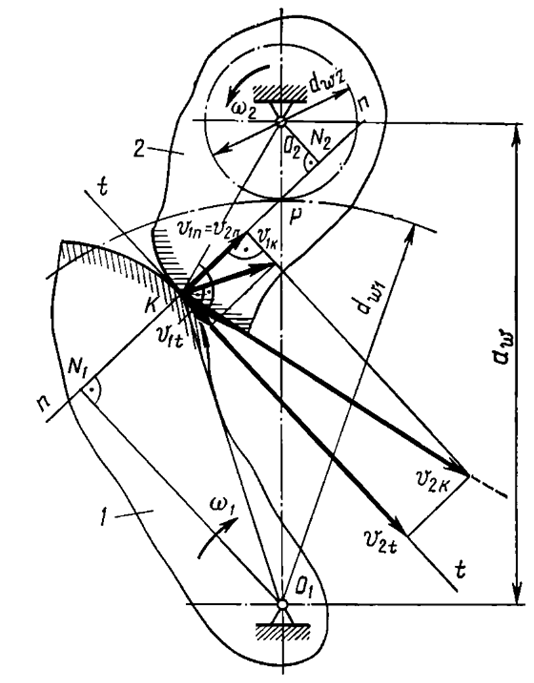
\includegraphics[width=0.6\textwidth]{OTZ.png}
	\caption{Основная теорема зацепления}
	\label{pic:OTZ}
\end{figure*}

Известна угловая скорость $ \omega_1 $ зубчатого колеса 1, а следовательно, и окружные скорости точек профиля его зуба, в том числе и точки $ K $ касания профилей зубьев, $ v_{1K} = \omega_1 O_1 K $. 
Для точки $ K $ профиля зуба ведомого колеса известно направление окружной скорости $ v_{2K} $, оно перпендикулярно радиусу $ O_2 K $. Из очевидного условия, что проекции скоростей соприкасающихся точек $ K $ профилей зубьев колёс 1 и 2 на общую нормаль $ n-n $ должны быть одинаковы, т.е. $ v_{1n} = v_{2n}$, получаем:
\begin{equation*}
\omega_1 O_1 N_1 = \omega_2 O_2 N_2, \text{или}\, i=\dfrac{\omega_1}{\omega_2} = \dfrac{O_2 N_2}{O_1 N_1}.
\end{equation*}


Так как $ \triangle O_1 N_1 P \propto O_2 N_2 P $, то $ \dfrac{O_2 N_2}{O_1 N_1} = \dfrac{O_2 P}{O_1 P}$. Отсюда следует, что
\begin{equation*}
i=\dfrac{\omega_1}{\omega_2} = \dfrac{O_2 N_2 }{O_1 N_1} = \dfrac{O_2 P}{O_1 P}.
\end{equation*}

Для получения постоянного передаточного отношения на всём участке зацепления зубьев необходимо, чтобы $ i=\dfrac{\omega_1}{\omega_2} = \dfrac{O_2 P}{O_1 P} = const $. 
Таким образом, при передаче зацеплением общая нормаль к профилям зубьев в любой точке их касания при повороте колёс должна проходить через одну и ту же точку $ P $, которая делит межосевое расстояние $ a_w $ на отрезки, обратное отношение которых $ \dfrac{O_2 P}{O_1 P} $ равно передаточному отношению $ i=\dfrac{\omega_1}{\omega_2} $. Профили зубьев колёс передачи называют сопряжёнными, если они соответствуют основной теореме зацепления.

Определённым\marginnote{\allcaps{СКОЛЬЖЕНИЕ ПРОФИЛЕЙ}} недостатком зубчатых зацеплений является \allcaps{скольжение профилей зубьев}. Скорость скольжения $ v_\text{ск} $ профилей зубьев равна разности проекций скоростей контактирующих точек зубьев на направление касательной $ t-t $ к профилям в точке их касания: 
\begin{equation}
\label{eq:gears_skolzhenie}
v_\text{ск}=v_{1t} - v_{2t} = -PK (\omega_1 + \omega_2).
\end{equation}

\begin{marginfigure}
	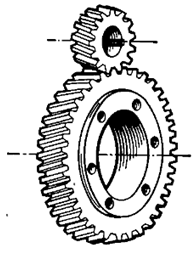
\includegraphics[width=0.6\linewidth]{osi5.png}
\end{marginfigure}

Из выражения \ref{eq:gears_skolzhenie} следует, что чем дальше от полюса $ P $ происходит контакт профилей зубьев, тем больше скольжение профилей.
Скольжение профилей отсутствует, когда точка их касания находится в полюсе $ P $. 
Полюс $ P $ является также мгновенным центром качения начальных окружностей, которые всегда касаются в полюсе. Это окружности диаметров $ d_{w1}, \, d_{w2} $. 
Таким образом:
\begin{equation*}
i=\dfrac{O_2 P}{O_1 P} = \dfrac{d_{w2}}{d_{w1}}.
\end{equation*}

\noindent
Следовательно, сопряжённые профили воспроизводят такую же передачу движения, как и исходные начальные окружности при их относительном качении без проскальзывания.

Наиболее распространённым профилем зубьев колёс, отвечающим требованиям основной теоремы зацепления, является эвольвента окружности.

\noindent
\textsc{Эвольвента}\marginnote{\allcaps{ЭВОЛЬВЕНТА}} --- кривая, представляющая собой траекторию движения любой точки прямой, перекатывающейся без скольжения по окружности.

\begin{figure}[h!]
	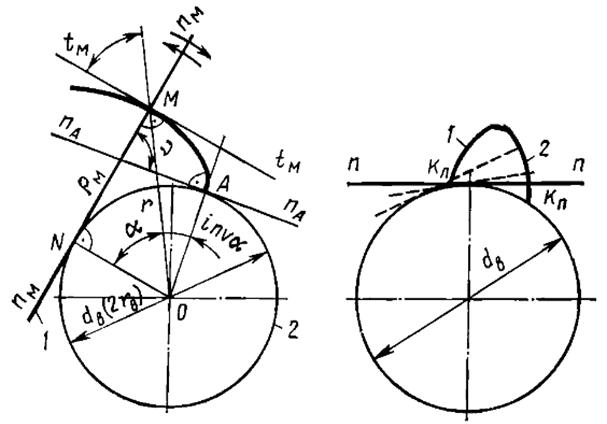
\includegraphics[width=0.8\textwidth]{evolventa1.png}
	\caption{Эвольвентный профиль зубчатого колеса}
	\label{pic:evolventa1}
\end{figure}

\begin{table}[ht]
	\centering
	\fontfamily{ppl}\selectfont
	\begin{tabular}{ll}
		\toprule
		Обозначение & Параметр \\ 
		\midrule
		$ m $ & модуль зацепления, [мм] \\
		$ z_1,\,z_2 $ & количество зубьев \\
		$ d_1,\,d_2 $ & диаметр делительной окружности, [мм] \\
		$ p=s+e $ & шаг зубьев, [мм] \\
		$ s $ & толщина зубьев, [мм] \\
		$ e $ & расстояние между профилями зубьев, [мм] \\
		$ d_a $ & диаметр окружности впадин, [мм] \\
		$ d_a $ & диаметр окружности вершин, [мм] \\
		$ h $ & высота зуба, [мм] \\
		$ h_f $ & высота головки зуба, [мм] \\
		$ \tau $ & центральный угол делительной окружности \\
		$ b $ & наименьшее расстояние между торцами зубьев \\
		\bottomrule
	\end{tabular}
	\caption{Основные параметры зубчатого колеса}
	\label{tab:parZ}
\end{table}


\newthought{Достоинства} прямозубой передачи:
\begin{itemize}
	\item высокое передаточное отношение (до 15);
	\item надежность и простота обслуживания;
	\item технологичность;
	\item малые габариты;
	\item высокий КПД (до 0,99);
	\item постоянство передаточного отношения $ i $;
	\item применение в широком диапазоне вращающих моментов, скоростей и передаточных отношений;
	\item малые нагрузки на валы и опоры;
	\item долговечность (до 50000 ч).
\end{itemize}

\newthought{Недостатки} прямозубой передачи:
\begin{itemize}
	\item высокие требования к точ­ности изготовления и монтажа и, как следствие, дороговизна;
	\item шум при работе со значительными скоростями;
	\item высокая жесткость, не позволяющая компенсировать динамические нагрузки;
	\item невозможность безступенчатого регулирования передаточного отношения.
\end{itemize}

\textsc{Методы нарезания зубьев}\marginnote{\allcaps{МЕТОДЫ НАРЕЗАНИЯ ЗУБЬЕВ}}:
\begin{itemize}
	\item метод деления (копирования);
	\item метод обката (огибания).
\end{itemize}

Для\marginnote{\allcaps{КОРРИГИРОВАННЫЕ\break ЗУБЧАТЫЕ\break ПЕРЕДАЧИ}} устранения подрезания зубьев применяют \textsc{корригированные зубчатые передачи}.
Корригирование определяется смещением режущего инструмента $ x = \xi m $ при нарезании зубьев:
\begin{itemize}
	\item отсутствие коррекции (нулевая передача): $ \xi_1 = \xi_2 = 0, \, \xi_\Sigma=0 $;
	\item высотная коррекция (равносмещённая передача): $ \xi_1 = -\xi_2 \neq 0, \, \xi_\Sigma=0 $;
	\item угловая коррекция, при которой происходит изменение угла зацепления: $ \xi_1 \neq \xi_2, \, \xi_\Sigma \neq 0 $, различают положительные ($\xi_\Sigma > 0 $) и отрицательные ($\xi_\Sigma < 0 $) передачи.
\end{itemize}

\marginnote{\allcaps{МАТЕРИАЛЫ ЗК}}

\section{Расчёт на прочность цилиндрических эвольвентных зубчатых колёс}

\section{Точность зубчатых колёс и передач}

\newthought{Точные приборные устройства}\marginnote{\allcaps{ТОЧНЫЕ ПРИБОРНЫЕ УСТРОЙСТВА}}~--- приборные устройства, точность работы которых регламентируется допусками.\marginnote{Допуск на точность обозначается $ [\delta_0 S] $}

Расчеты на точность подразделяются на:
\begin{itemize}
	\item прямой (проектный) -- определение точностных требований к составляющим устройствам, узлам и деталям;
	\item обратный (проверочный) -- определение погрешности ПУ на основе разработанных точностных требований к звеньям устройства.
\end{itemize}

Существует 12 степеней точности. В приборостроении обычно применяют 6-9 степени точности.

\newthought{Показатели точности} регулируются стандартами (контрольные комплексы):
\begin{itemize}
	\item \allcaps{кинематическая точность}\marginnote{\allcaps{КИНЕМАТИЧЕСКАЯ\break ТОЧНОСТЬ}} --- наибольшая погрешность функции положения при работе передачи в одном направлении или наибольшая погрешность $ i $;
	\item \allcaps{плавность работы}\marginnote{\allcaps{ПЛАВНОСТЬ РАБОТЫ}} --- плавность изменения кинематической погрешности – колебания скорости за один оборот, источник динамической нагрузки;
	\item \allcaps{пятно контакта}\marginnote{\allcaps{ПЯТНО КОНТАКТА}} --- полнота прилегания зубьев и концентрация нагрузки на их поверхности;
	\item \allcaps{боковой зазор}\marginnote{\allcaps{БОКОВОЙ ЗАЗОР}} между работающими профилями зубев --- для компенсации температурных деформаций, смазки, погрешностей сборки и изготовления; боковой зазор нормируется независимо от степени точности зубчатых колёс и передач, определение которого основано на величине минимального гарантированного бокового зазора $ j_{n\,min} $.
\end{itemize}

Для всех видов передач предпочтительными являются функциональные показатели  и суммарное пятно контакта.

\section{Проектный расчёт зубчатых передач на прочность}
\subsection{Виды разрушений зубчатых колёс}
Основными видами разрушения зубчатых колёс являются излом от напряжений изгиба в материале зубьев и выкрашивание рабочих поверхностей зубьев от контактных напряжений, если в обоих случаях напряжения превосходят допускаемые значения. 
Износ от контактных напряжений является характерным для зубчатых колёс, находящихся в масле (закрытые передачи).
Масло, находящееся в месте контакта зубьев, под давлением заполняет поверхностные микротрещины в зубьях, вызывая постепенное разрушение.

\begin{marginfigure}
	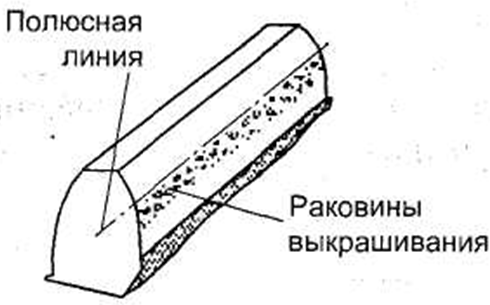
\includegraphics[width=1\linewidth]{polomkaZ1.png}
\end{marginfigure} 
\textsc{Выкрашивание} поверхностных слоев зубьев характерно для закрытых хорошо смазываемых передач. 
При циклическом нагружении на поверхности зубьев у полюсной линии разрастаются микротрещины, что приводит к образованию оспинок, переходящих в раковины. Выкрашивание может быть ограниченным или прогрессирующим.

\begin{marginfigure}
	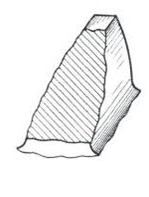
\includegraphics[width=0.6\linewidth]{polomkaZ.png}
\end{marginfigure}
\textsc{Поломка зубьев} может носить усталостный характер или являться следствием значительных перегрузок. При циклическом нагружении микротрещины у корня зуба разрастаются, что приводит к излому по сечению у основания зуба прямозубых колёс или по косому сечению – косозубых и шевронных колёс.

\begin{marginfigure}
	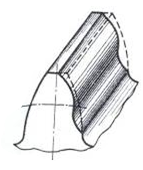
\includegraphics[width=0.6\linewidth]{polomkaZ2.png}
\end{marginfigure}
\textsc{Абразивный износ} характерен для открытых передач, а также закрытых, работающих при скудной смазке и наличии абразивов.

\begin{marginfigure}
	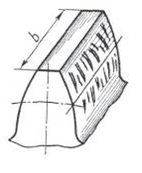
\includegraphics[width=0.6\linewidth]{polomkaZ3.png}
\end{marginfigure}
\textsc{Заедание} характерно для высоконагруженных передач. При высокой удельной нагрузке происходит разрыв масляной плёнки, нагрев и схватывание сопряжённых поверхностей с образованием следов задира в направлении скольжения зубьев.

Цель проектного расчёта зубчатых передач на прочность~--- определение модуля зацепления и размеры передач, обеспечивающие их работоспособность в течение заданного срока службы. 

В зависимости от вида разрушения и условий работы передачи необходимо проводить расчёт на изгибную прочность и расчёт зубьев на контактную прочность.

Расчётные формулы содержат ряд коэффициентов.
Эти коэффициенты, общие для расчёта на изгибную прочность и на контактные напряжения, обозначают $ K $.
Коэффициенты, характерные только для расчёта на изгиб, обозначают $ Y $.
Чтобы показать, что расчёт на изгибную прочность проводится по опасному сечению, находящемуся в основании ножки зуба, применяют букву $ F $, т.е. $ Y_F $.
Коэффициенты, характерные только для расчёта по контактным напряжениям, обозначают $ Z $.
Индекс $ H $ у коэффициентов $ Z_H $ при расчёте на контактную прочность введён в честь Герца.
\subsection{Исходные соотношения между окружными и нормальными силами и давлениями в прямозубых эвольвентных зубчатых передачах}
Формулы для расчёта на прочность зубчатых колёс содержат моменты сил, выраженные через окружные силы.
Изгибные и контактные напряжения рассчитывают по нормальным силам и давлениям.
Для вывода расчётных формул необходимо учитывать соотношения между окружными и нормальными силами и давлениями.
Значения нормальных сил и давлений определяют по моменту нагрузки $ M_2 $, приложенному к ведомому колесу:
\begin{equation}
F_n = \dfrac{2 M_2 K}{d_2 \cos\alpha}.
\end{equation}



\section{Косозубые зубчатые колёса}
\newthought{Косозубые колёса}\marginnote{\allcaps{КОСОЗУБЫЕ КОЛЁСА}} применяют для увеличения плавности хода и при повышенных нагрузках вместо прямозубых.

\newthought{Достоинства}:
\begin{itemize}
	\item высокий коэффициент торцевого перекрытия , что обеспечивает высокую плавность хода, повышенную прочность, снижение шума, уменьшение динамических нагрузок
	\item возможность подбора заданного межосевого расстояния, когда известно передаточное отношение и задан стандартный модуль, но нет возможности подобрать прямозубое колесо
	\item возможность работы при повышенных окружных скоростях~(до~30~м/с)
\end{itemize}

\newthought{Недостатки}: появление осевой силы, которая может быть компенсирована использованием шевронной передачи.
